\documentclass[11pt]{article}

\usepackage{graphicx}
\usepackage{authblk}
\usepackage{indentfirst}
\usepackage{amsmath}
\usepackage{booktabs}
\usepackage{hyperref}
\usepackage{enumitem}
\usepackage{float}
\usepackage[margin=0.9in]{geometry}

\usepackage{titlesec}
\usepackage{multicol}
\addtolength{\textheight}{0.55in}
\titlespacing*{\section}{0pt}{1.0em}{0.35em}
\titlespacing*{\subsection}{0pt}{0.7em}{0.25em}
\setlength{\abovedisplayskip}{5pt}
\setlength{\belowdisplayskip}{5pt}
\setlength{\textfloatsep}{8pt}
\setlength{\intextsep}{8pt}

\hypersetup{colorlinks=true, linkcolor=blue, urlcolor=blue, citecolor=blue}

\raggedbottom
\clubpenalty=10000 \widowpenalty=10000
\begin{document}

\title{CHEM 396 Final Report\\[0.3em]
\large Melt-Quench Molecular Dynamics of Amorphous Silicon with Moment Tensor Potentials}
\author{William R. Homier}
\affil{Department of Physics, McGill University}
\affil{Supervisor: Prof.\ Lena Simine \quad Co-mentor: Ata Madanchi}
\date{August 28, 2026}
\setcounter{Maxaffil}{0}
\renewcommand\Affilfont{\itshape\small}
\maketitle
\thispagestyle{empty}

\noindent\rule{\textwidth}{0.4pt}
\begin{abstract}
    \noindent This report covers a project on building models of amorphous silicon by melt-quench molecular dynamics with Moment Tensor Potentials. Five silicon MTPs were tested: two melt-stable unpruned models at levels 22 and 26, and three pruned variants of increasing cost. The first deliverable was a working toolchain on Narval. Both supplied LAMMPS build scripts were broken and were diagnosed and repaired, giving a CPU build used for all production runs and a Kokkos GPU build validated on a Lennard-Jones benchmark. A 216-atom system was then run through a common melt-quench protocol for all five: a 30~ps ramp to 2500~K, a 1~ns hold, a 2.2~ns quench at 1~K/ps, and a 150~ps equilibration at 300~K. Level 26 was held for 0.4~ns and not quenched, to save compute time, so four were carried through to final structures. Three results came out of this. First, every pruned potential survived the 2500~K hold with no instability and no energy drift, which was not expected, and pruning bought a speedup of 1.6 to 11.7 times in the hold and 1.6 to 10.7 times in the quench. Second, all four quenched structures are properly amorphous: the second peak of $g(r)$ survives at 3.88~\AA{} while the third crystalline shell at 4.50~\AA{} never appears, the mean squared displacement plateaus at 0.05~\AA$^2$, and the tetrahedral order parameter sits at 0.93 against 0.99 for the crystal and 0.49 for the liquid. Third, the cost of pruning shows up in the defect count, which runs from 3.7\% for unpruned level 22 to 8.0\% for the cheapest pruned potential, with over-coordination dominating in every run. A crystallinity check in OVITO gives a time-averaged 4.5\% for level 22, carried by a single 17-atom diamond motif that flickers in and out of classification as the atoms vibrate. The structures are ready to hand to MAP.
\end{abstract}
\noindent\rule{\textwidth}{0.4pt}
\clearpage

\thispagestyle{empty}
\pagenumbering{gobble}
{\hypersetup{linkcolor=black}\tableofcontents}
\clearpage
\pagenumbering{arabic}
\setcounter{page}{1}

% ===========================================================
\section{Introduction}

Amorphous silicon (a-Si) lacks the long-range order of crystalline silicon (c-Si). Most atoms are still bonded to four neighbours in roughly tetrahedral arrangements, but bond lengths and angles vary rather than being fixed. a-Si is used in solar cells, thin-film transistors and battery anodes, and its properties depend strongly on coordination defects, meaning atoms with too few or too many bonds.

Simulating a-Si requires a model of the forces between atoms. Density functional theory is accurate but expensive. Empirical potentials are cheap but locked into a fixed functional form, and a pair potential such as Lennard-Jones cannot describe silicon at all, since silicon demands specific bond angles and Lennard-Jones has no angular term. Machine-learned potentials sit in between. They still have a definite functional form, but it is a systematically expandable basis rather than a hand-chosen physical one, and the coefficients are fitted to DFT energies and forces instead of to a few experimental numbers. This project uses one of them, the Moment Tensor Potential (MTP).

The specific question is what pruning costs. A pruned MTP drops basis functions from the energy expansion so that it runs faster, and where that breaks down could not be predicted in advance. Liquid silicon at 2500~K visits geometries very unlike the crystal structures that fill most training sets, so a stripped-down basis is exactly where trouble would be expected. Running the same melt-quench with each potential turns that expectation into a measurement.

\subsection{Objectives}
\begin{enumerate}[nosep]
    \item Build a working MTP-enabled LAMMPS toolchain on Narval, CPU and GPU, and validate it.
    \item Characterize the five supplied potentials for cost, melt stability and preferred volume.
    \item Run the same melt-quench protocol with each potential.
    \item Characterize the resulting networks against Zongo et al.\ (2025) and experiment.
    \item Hand the structures to MAP.
\end{enumerate}
Objectives 1 to 3 are complete. Objective 4 is mostly complete: the structures are characterized and compared against Zongo et al.\ and experiment, but bond angle and ring statistics were not computed (Section~\ref{sec:gaps}). Objective 5 is not done. MAP is installed and configured on Narval but has not yet been applied to these structures, so it is reported as future work. The interim report folded MAP into its objective 4; it is split out here so the two can be reported separately.

\subsection{Relation to the interim report}
The interim report of July 28 covered objectives 1 and 2 and the melt. This report is self-contained, but anything already shown there is stated as a result, not worked through again: the build faults, the atom-type mapping, the equilibrium volume, the parallel scaling and the volume mismatch between potential families appear in Section~\ref{sec:carried} in compressed form. Everything from the 2500~K hold onward is new. One protocol change was made after the interim. The interim planned a handoff in which a melt-stable potential ran the melt and hold and a pruned potential ran the quench. Once the pruned potentials were found to be stable in the melt (Section~\ref{sec:melt}), each potential instead ran its own hold and its own quench, which keeps the comparison between potentials clean instead of mixing in a shared starting liquid.

% ===========================================================
\section{Background}

\subsection{Amorphous silicon}
c-Si is diamond cubic, with four neighbours per atom at a bond length of 2.35~\AA{} and angles of $109.5^\circ$. In a-Si the local bonding survives but the periodicity is gone: bond lengths and angles spread out, and a few percent of atoms become coordination defects, threefold being a dangling bond and fivefold a floating bond. The standard picture is the continuous random network, in which nearly every atom is still fourfold and the disorder is in the geometry rather than in broken bonds. Experimental a-Si has a mean coordination of 3.88 and a density of 2.28~g/cm$^3$, against exactly 4 and 2.33 for the crystal, with bond angles spread around $109.5^\circ$ at an RMS width near $10^\circ$. Melt-quench MD traps defects, more so at faster cooling, and it is also the route reported to trap crystalline grains (Treacy and Borisenko, 2012; Rosset et al., 2025), so the structures had to be checked for residual crystallinity rather than assumed clean (Section~\ref{sec:crystal}).

\subsection{Moment Tensor Potentials}
An MTP (Shapeev, 2016) writes the energy as a linear sum over invariant basis functions built from moment tensors of each atom's neighbourhood, with coefficients fitted to DFT energies and forces, at a cost linear in atom count. The \emph{level} is how many basis functions the sum uses: a higher level covers more geometries and costs more per force call, which is why level 26 is richer and slower than level 22.

Pruning comes from the other direction and is the subject of this report. Many basis functions barely affect the structures that actually occur, so they are dropped from an already-trained model, giving nearly the same fit with a shorter sum and fewer operations per atom per timestep. \texttt{pruned\_1} keeps the least of the basis and is cheapest, \texttt{pruned\_3} keeps the most. Nothing says the dropped terms stay unimportant away from the training data, and a 2500~K liquid is a long way from it, so the pruned potentials were expected to be the fragile ones. Meng et al.\ (2026) also added a Kokkos GPU version targeting roughly 2000 atoms or more per GPU; it was built here but the production cell is far too small to benefit (Section~\ref{sec:disc_gpu}).

\subsection{Benchmark study}
Zongo et al.\ (2025) is the reference for comparison. It builds seven a-Si models of 216 to 4096 atoms with the unified Si/O/SiO$_2$ MTP of Zongo et al.\ (2024) driven by the activation-relaxation technique, reaching defect levels below 2\%, bond angles centred on $109.5^\circ$ with a $10^\circ$ spread, and zero crystallinity in the four models built from a random fill with no MD prerun. Their conclusion is that melt-quench MD traps crystalline grains where ARTn does not, which makes the paper both the structural target here and a warning about the failure mode to check for. Their two 216-atom melt-quench models report 1.85\% and 1.86\% defects, and 1.85\% is the figure used for comparison.

\subsection{MAP}
The Morphological Autoregressive Protocol (Madanchi et al., 2024) generates disordered structures one grid point at a time, each conditioned only on already-placed neighbours inside a finite correlation length, at linear cost. A follow-up (Madanchi and Simine, 2026) runs the trained model in reverse as an anomaly detector, scoring each particle by how likely its local environment is, with dips matching about 88\% of independently identified rearrangement events. That reverse use is what this project feeds into.

% ===========================================================
\section{Methodology}

\subsection{Simulation protocol}
Five potentials were provided. \texttt{22.almtp} and \texttt{26.almtp} are melt-stable and unpruned; \texttt{pruned\_1} to \texttt{pruned\_3} are pruned in order of increasing cost and accuracy. Each ran the same five stages: start from a 216-atom diamond lattice, $3\times3\times3$ conventional cells at $a = 5.431$~\AA; ramp 300~K to 2500~K over 30~ps; hold at 2500~K for 1~ns to erase the memory of the crystal; cool to 300~K at 1~K/ps, which is 2200~ps; equilibrate at 300~K for 150~ps. Every stage ran under NPT at 0~bar, isotropic, periodic, \texttt{units metal}, 1~fs timestep, neighbour skin 0.3~\AA, delay 5, check every step, thermo output every 5 steps, dumps every 100 and restarts every $10^5$. All production runs used the CPU build on 8 MPI tasks, launched with \texttt{srun} under \texttt{--ntasks=8 --mem-per-cpu=2G}. Each stage is a single \texttt{fix npt ... iso 0.0 0.0 1.0} with a 0.1~ps thermostat damping followed by a \texttt{run}, with the melt built from \texttt{lattice diamond 5.431} and later stages resumed through \texttt{read\_data}. Full input scripts and SLURM submission scripts are in the project code directory, and the submission scripts also appear in the interim report.

LAMMPS has no cooling-rate command. \texttt{fix npt} ramps linearly from a start to a target temperature over whichever \texttt{run} follows it, so the rate is set by the run length:
\begin{equation}
    \text{rate} = \frac{\Delta T}{N_{\text{steps}}\,\Delta t}.
    \label{eq:rate}
\end{equation}
At 1~K/ps a 2200~K drop is $2.2\times10^6$ steps. One consequence matters on restart: the ramp is defined relative to the current \texttt{run} and not to an absolute timestep, so a resumed quench needs its start temperature and remaining step count recomputed by hand. The 216-atom cell matches the smallest models of Zongo et al.

\subsection{Structural observables}
Structural numbers are averaged over the last 50~ps of the 300~K equilibration; the MSD uses the full block. The radial distribution function $g(r)$ is the probability of finding another atom a distance $r$ away, normalized so that a uniform gas gives 1. Its first peak is the bond length, its first minimum sets the bonding cutoff, and the behaviour past the second peak separates a glass from a crystal. Coordination number is the neighbour count inside that first minimum, cutoff 2.85~\AA{} to match the OVITO analysis of Zongo et al., or 3.15~\AA{} in the liquid. The liquid value was read off the melt, and the equilibrated holds put the first minimum slightly further out at 3.24 to 3.32~\AA, so liquid coordination is a small undercount; all five potentials use the same cutoff, so the comparison between them is unaffected. The tetrahedral order parameter is
\begin{equation}
    q = 1 - \frac{3}{8}\sum_{i<j}\left(\cos\theta_{ij} + \tfrac{1}{3}\right)^{2},
    \label{eq:top}
\end{equation}
taken over the four nearest neighbours, where $\theta_{ij}$ is the angle at the central atom; a perfect tetrahedron gives 1 and a random arrangement gives 0, and it ignores bond length. Note that it uses four neighbours whatever the real coordination, so a fivefold atom is scored on the best four of its five bonds and reads more tetrahedral than the site actually is. That bias runs the same way as the over-coordination reported below, so $q$ should be read next to the defect fraction and not on its own. The mean squared displacement $\langle|\mathbf{r}(t)-\mathbf{r}(0)|^2\rangle$ plateaus in a solid, because atoms vibrate around fixed sites, and rises linearly in a liquid with a slope giving $D$ through $\mathrm{MSD}=6Dt$. Density is $\rho=Nm/V$ with $V$ from the NPT run.

% ===========================================================
\section{Results}

\subsection{Toolchain and settings used throughout}
\label{sec:carried}
\label{sec:builds}
The toolchain and run settings were set before the interim report, which lists them in full. They are stated here as results, since everything below depends on them.

Neither build script produced a working binary. Five faults were found and fixed: an architecture flag causing ``Illegal instruction'' on nodes other than the build node, an inverted conditional that skipped the MTP sources, stale nested CMake caches that \texttt{--fresh} does not clear, an uncopied \texttt{KOKKOS} folder, and a Kokkos CUDA backend that was never enabled. The result is a CPU build used for every production run and a Kokkos GPU build, validated together on the 13{,}500-atom Lennard-Jones benchmark at 4~min 16~s on one CPU core against 15.6~s on one A100, about $16\times$. That benchmark is 60 times larger and uses a far cheaper potential per atom, so the speedup does not carry over to production (Section~\ref{sec:disc_gpu}).

Four other settings were then fixed. Type 1 in the potential file is silicon and type 2 oxygen, settled by running the lattice as each: type 1 was stable at 2.272~g/cm$^3$ against 2.33 for c-Si, while type 2 started at $-2.24\times10^6$~bar and collapsed at once. NPT at 300~K and 0~bar settles the box at 4433~\AA$^3$, so $a = (4433/27)^{1/3} = 5.476$~\AA, 0.83\% above the experimental 5.431 and the direction expected for a potential trained on PBE data. Eight MPI tasks is the working core count, from wall times of 22:55, 5:07 and 2:43 on 1, 4 and 8 cores; 64 fails, since the MTP cutoff is 5.7~\AA{} and 64 subdomains of a 16.4~\AA{} box are only 4~\AA{} wide. And the two families prefer different volumes, with \texttt{pruned\_1} holding $-12{,}400$~bar in the box where \texttt{22.almtp} sits at zero pressure. Running NPT throughout lets the barostat absorb that, and the effect returns in the final density (Section~\ref{sec:density}).

One run failed along the way. The first \texttt{pruned\_3} quench stopped at step $2.94\times10^5$ with an I/O error on the dump write. The error was \texttt{EIO} rather than \texttt{EDQUOT} and scratch stood at 351~MB of a 20~TB quota, so the cause was a transient Lustre fault rather than a full filesystem. The run was repeated and finished 5\% under its projected 15.3~h. It is why restart files were written every $10^5$ steps thereafter.

\subsection{Computational cost}
\label{sec:cost}

\begin{table}[H]
\centering\footnotesize
\begin{tabular}{lcccc}
\toprule
Potential & Hold (steps/s) & Rel.\ to 22 & Quench (steps/s) & Rel.\ to 22 \\
\midrule
\texttt{22.almtp}  & 26.2  & $1.00\times$ & 29.2  & $1.00\times$ \\
\texttt{26.almtp}  & 10.4  & $0.40\times$ & N/A    & N/A \\
\texttt{pruned\_1} & 307.2 & $11.7\times$ & 313.5 & $10.7\times$ \\
\texttt{pruned\_2} & 110.7 & $4.2\times$  & 106.9 & $3.7\times$ \\
\texttt{pruned\_3} & 42.6  & $1.6\times$  & 47.8  & $1.6\times$ \\
\bottomrule
\end{tabular}
\caption{Throughput for 216 atoms on 8 CPU cores. Hold figures come from the 2500~K stage; quench figures come from the 300~K block only, since LAMMPS prints one timing summary per \texttt{run}. Extrapolated to $10^6$ steps, a 1~ns hold takes 10.6~h for level 22, 26.7~h for level 26, 54~min for \texttt{pruned\_1}, 2.5~h for \texttt{pruned\_2} and 6.5~h for \texttt{pruned\_3}.}
\label{tab:cost}
\end{table}

The interim report projected a 9.1~h hold for level 22 from benchmarks on a static 300~K crystal, and noted a hot liquid would run slower because it rebuilds neighbour lists constantly. The measured hold took 10.6~h, 16\% over, in the predicted direction and size, with 30{,}215 neighbour rebuilds against none in the benchmark runs. Level 26 costs 2.53 times level 22 in the hold and 2.49 times in the melt. The same factor in both means the extra cost is per force call and does not depend on whether the system is a hot liquid or a cold crystal. Pruning runs the other way and buys back 1.6 to 11.7 times. The quench speedups come out slightly smaller than the hold values, because force evaluation is not the only cost: cores also spend time exchanging atoms, and that cost does not shrink when the potential gets cheaper, so its share of the run grows.

\subsection{Melt stability and the potential handoff}
\label{sec:melt}
All five potentials sat through the 2500~K hold with no blow-up, no dangerous neighbour-list builds and no drift in the potential energy over $10^6$ steps, with absolute energies matching level 22 to within 0.002\%. The pruned variants were expected to misbehave at melt temperatures and did not, which is the first main result, and a useful kind of negative result. The \texttt{26.almtp} hold was stopped at 0.4~ns because a full nanosecond at 2.53 times the cost was not worth the compute time, not because anything went wrong.

Four independent signatures agree that the system melted. Mean coordination goes from 4.000 to 5.968, $q$ from 0.993 to 0.498, and the box contracts by 4.2\%, from 4500 to 4310~\AA$^3$ between the first 2~ps and the last 3~ps of the ramp, the correct sign since liquid silicon is denser than the crystal. That end-of-ramp liquid is 2.337~g/cm$^3$ where the same potential gives 2.32 after the full hold; a liquid that has existed for 4~ps is still relaxing, so the hold value is the one used in Section~\ref{sec:density}. The MSD stays below 1~\AA$^2$ for the first 25~ps, rising only as the atoms vibrate harder, then kicks upward at 25.6~ps and climbs linearly to 111.4~\AA$^2$ over the remaining 4.4~ps of the ramp; level 26 gives 107.5~\AA$^2$ from 25.7~ps, one dump frame apart. Melting at 25.6~ps is 2177~K on the ramp, well above the experimental 1687~K, which is expected rather than a fault: a defect-free periodic crystal has no surface, grain boundary or vacancy to nucleate from, so it superheats until it melts homogeneously throughout the bulk. The 111.4~\AA$^2$ figure covers the end of the ramp only, not the hold, and the slope it implies, $D=\mathrm{MSD}/6t=4.2\times10^{-8}$~m$^2$/s, matches the 3.7 to $5.3\times10^{-8}$ measured directly in the holds.

Because the pruned potentials held, each one could run its own melt and quench, so it is fair to ask whether the starting structure biases the comparison. It does not, because the liquid forgets: at $D\approx4\times10^{-8}$~m$^2$/s over 1~ns, $\sqrt{6Dt}\approx155$~\AA, roughly ten box lengths. The liquids confirm this. Across all five potentials the first peak of $g(r)$ sits at 2.44~\AA, mean coordination spans 5.912 to 5.970 (1.0\%) and $q$ spans 0.4821 to 0.4975 (3.1\%). The leftover differences do not line up with pruning level, since \texttt{pruned\_3} is the most accurate variant and gives the highest coordination while \texttt{pruned\_2} gives the lowest, so this is sampling noise rather than the pruning hurting anything.

\subsection{Structure of the quenched solid}

\begin{table}[H]
\centering\footnotesize
\begin{tabular}{lcccccccc}
\toprule
Potential & $r_1$ & $r_{\min}$ & $r_2$ & $\bar{n}$ & defects & $q$ & MSD & $\rho$ \\
 & (\AA) & (\AA) & (\AA) & & (\%) & & (\AA$^2$) & (g/cm$^3$) \\
\midrule
\texttt{22.almtp}  & 2.36 & 2.84 & 3.88 & 4.019 & 3.7 & 0.9304 & 0.050 & 2.2491 \\
\texttt{pruned\_1} & 2.36 & 2.92 & 3.88 & 4.081 & 8.0 & 0.9205 & 0.055 & 2.2881 \\
\texttt{pruned\_2} & 2.36 & 2.92 & 3.88 & 4.040 & 4.2 & 0.9302 & 0.050 & 2.2479 \\
\texttt{pruned\_3} & 2.36 & 2.84 & 3.88 & 4.013 & 4.0 & 0.9286 & 0.047 & 2.2613 \\
\bottomrule
\end{tabular}
\caption{The quenched solid at 300~K. $r_1$, $r_{\min}$ and $r_2$ are the first peak, first minimum and second peak of $g(r)$. Coordination uses a 2.85~\AA{} cutoff and ``defects'' is the fraction of atoms that are not fourfold, both over the last 50~ps. MSD is the plateau value. Reference values: bond length 2.35~\AA{} in c-Si and mean coordination 3.88 and density 2.28~g/cm$^3$ in experiment; $q = 0.99$ and $0.49$ are this work's own crystal and liquid values, not literature.}
\label{tab:quench}
\end{table}

\begin{figure}[H]
    \centering
    \begin{minipage}{0.41\textwidth}
        \centering
        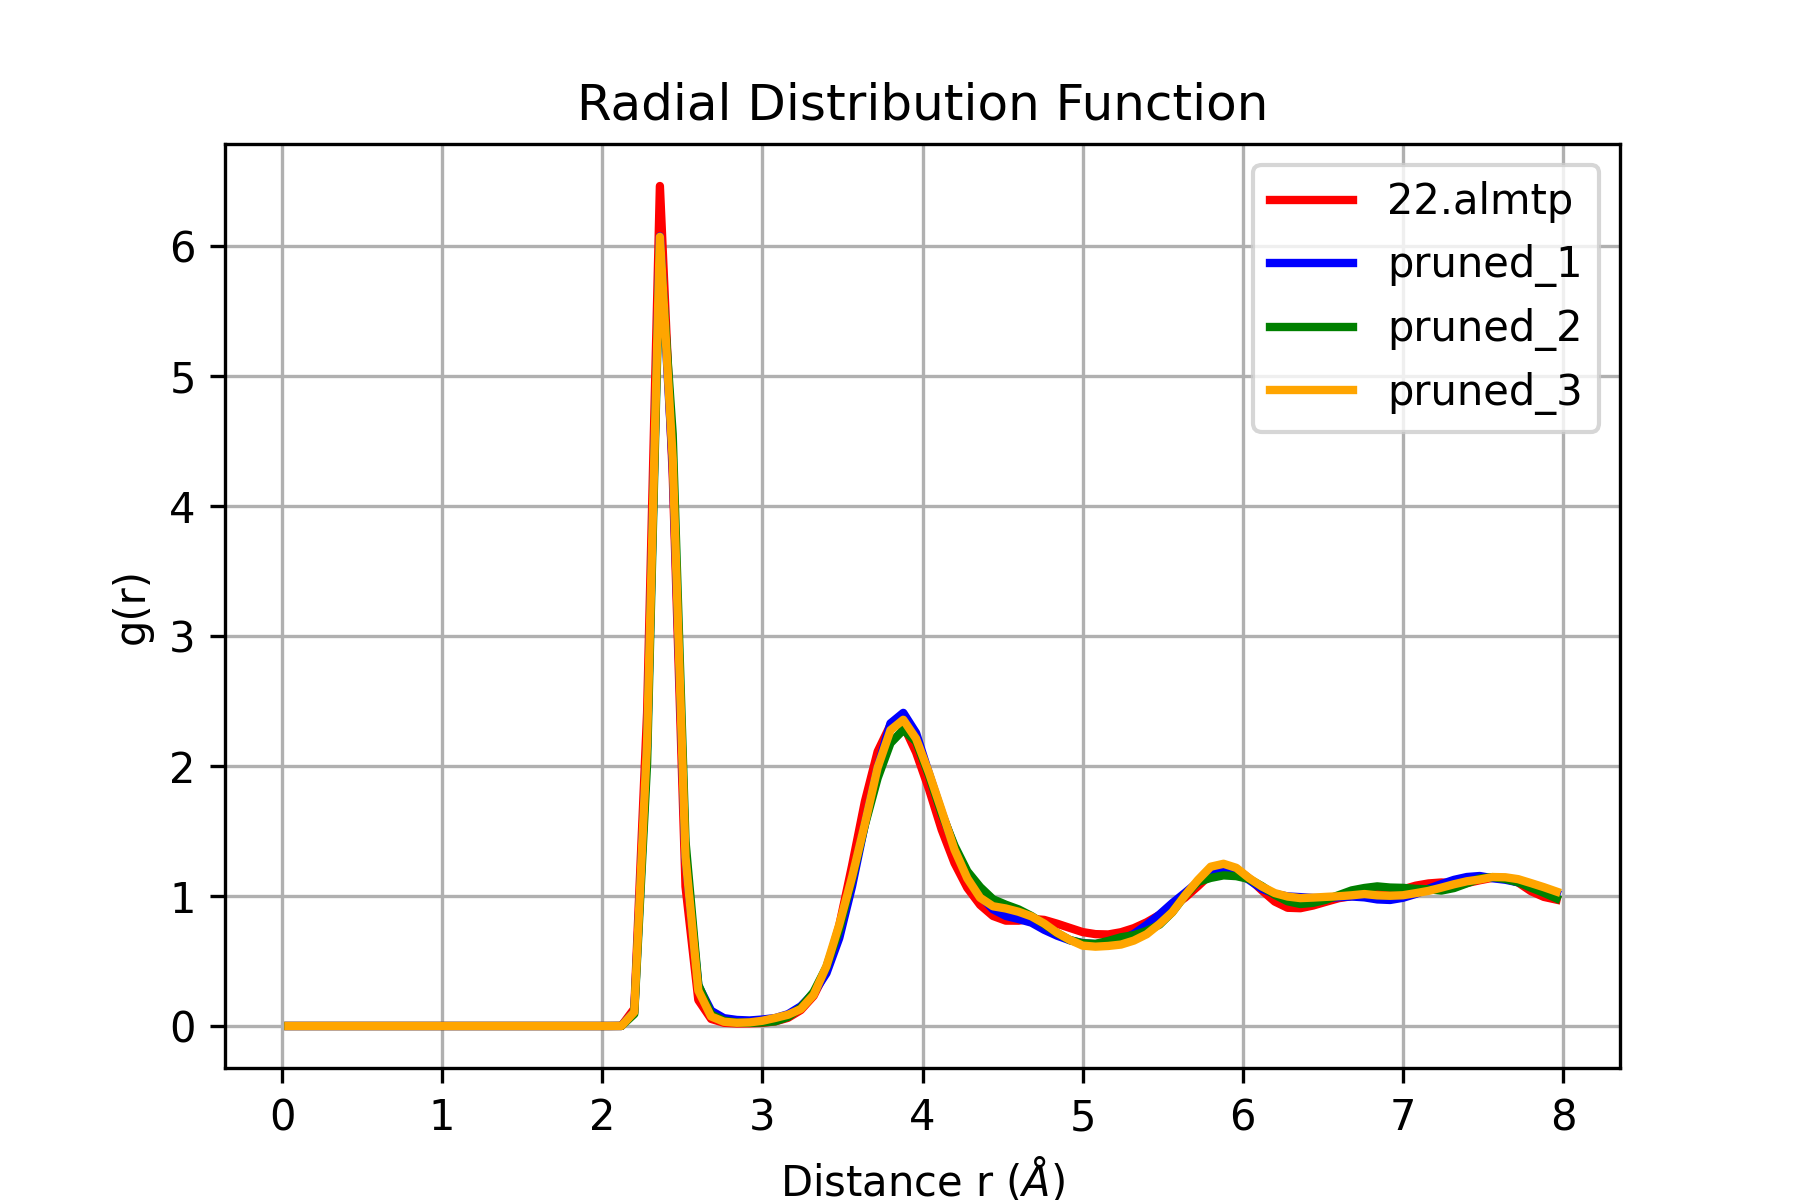
\includegraphics[width=\linewidth]{../python/radial_dist_fct/quench_hold_all_rdf_output.png}
    \end{minipage}
    \hfill
    \begin{minipage}{0.41\textwidth}
        \centering
        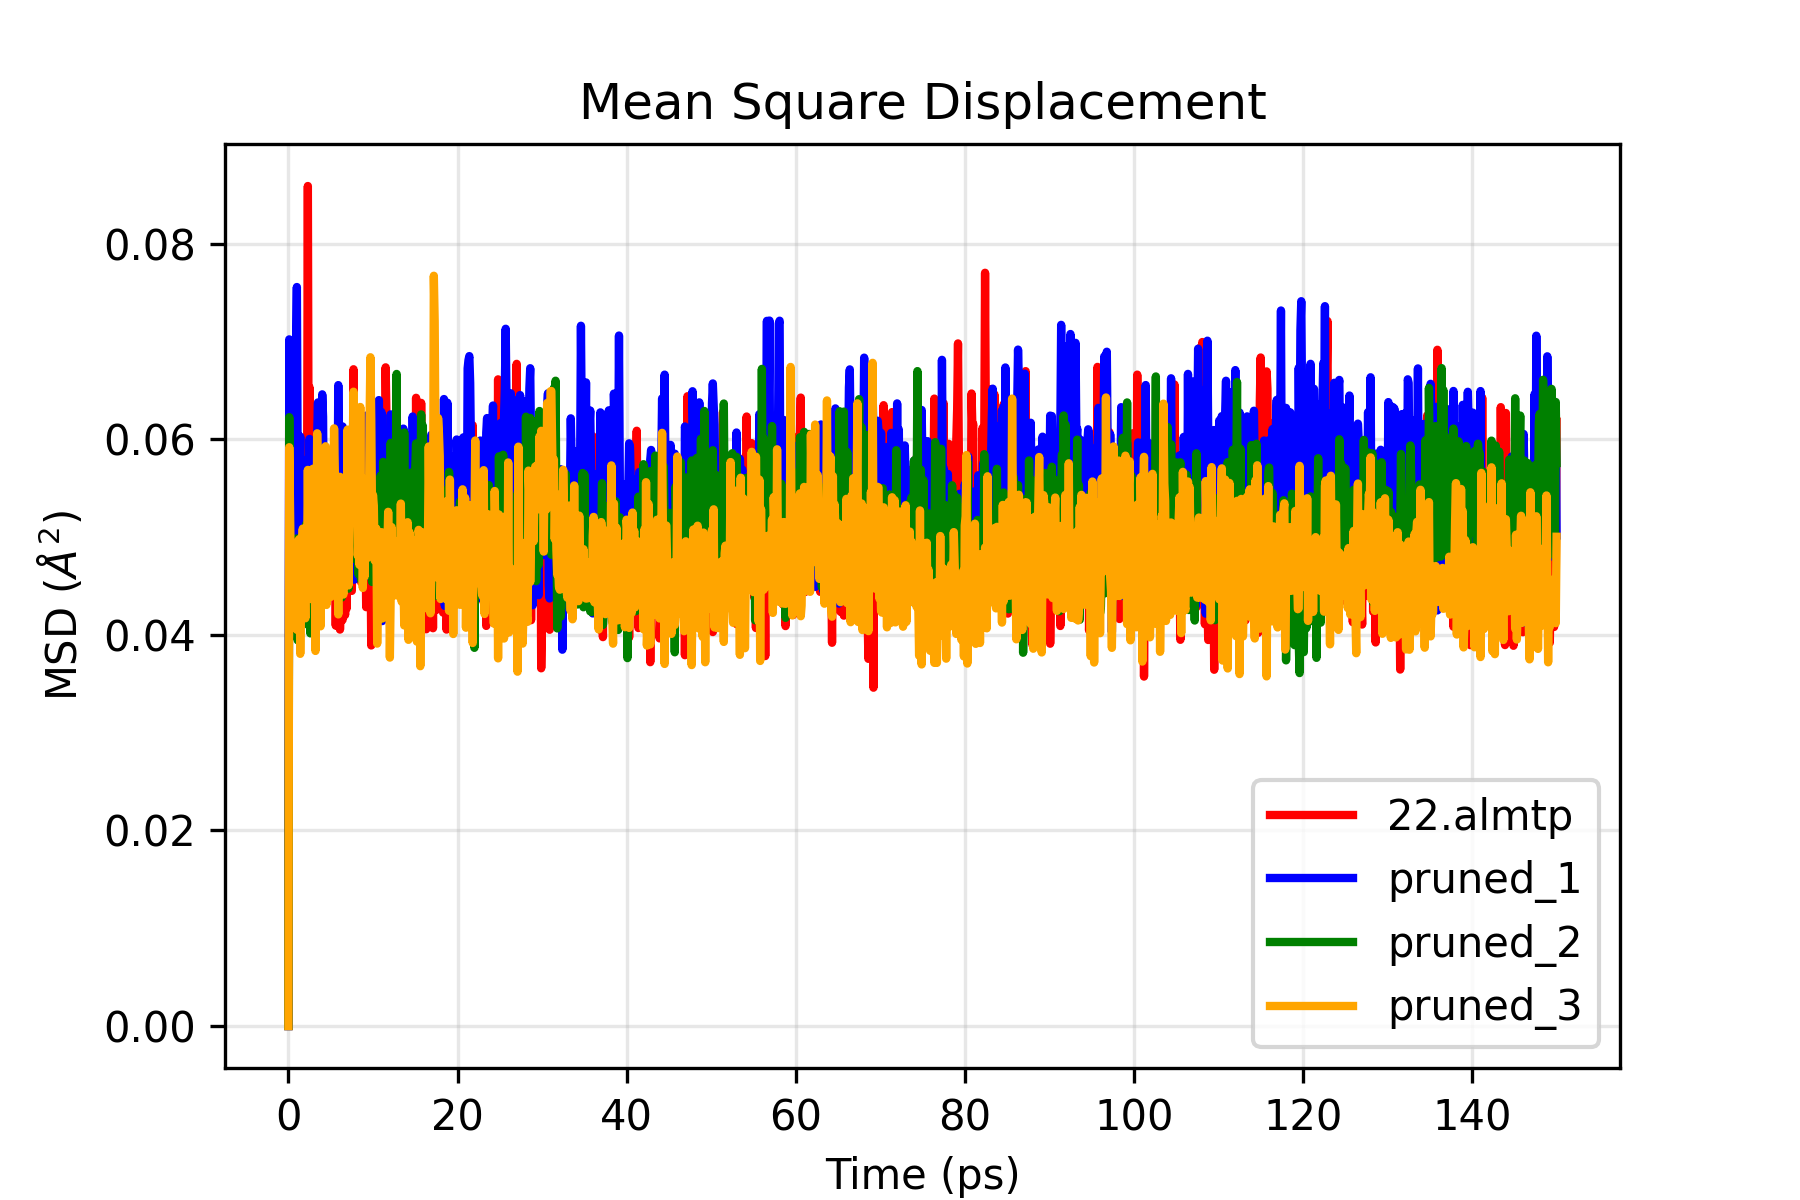
\includegraphics[width=\linewidth]{../python/msd/quench_hold_all_msd_output.png}
    \end{minipage}
    \caption{Left: radial distribution functions of the four quenched structures at 300~K, over the last 50~ps. Right: mean squared displacement over the full 150~ps equilibration.}
    \label{fig:quench}
\end{figure}

The clearest sign is what the second and third peaks do together. All four structures keep the second peak at 3.88~\AA{} and none show the crystalline third shell at 4.50~\AA, where the liquid had nothing at all beyond 3.5~\AA. That is what a continuous random network looks like: the tetrahedral geometry survives out to second neighbours, but the periodic order that would place atoms in a well-defined third shell is gone. The 2.85~\AA{} cutoff taken from Zongo et al.\ lands close to the measured first minimum, 2.84~\AA{} for two potentials and 2.92~\AA{} for the other two. For \texttt{pruned\_1} and \texttt{pruned\_2} the fixed cutoff therefore sits 0.07~\AA{} inside their own minimum, which if anything undercounts their neighbours; recounting each structure at its own minimum was not done and is listed as a gap in Section~\ref{sec:gaps}.

The MSD plateaus at 0.047 to 0.055~\AA$^2$ for the full 150~ps. Fitting a slope to the plateau bounds the apparent $D$ at order $10^{-14}$~m$^2$/s, six orders of magnitude below the melt, and one of the four slopes comes out negative, so it is a ceiling rather than a real measurement. The individual atoms agree: displacement from the mean position gives an amplitude of 0.139 to 0.150~\AA{} across the four potentials, RMS 0.152 to 0.166~\AA, and the largest single excursion over the whole 150~ps is 1.61, 1.47, 1.34 and 1.89~\AA, all below the 2.35~\AA{} bond length. Those two numbers are the same measurement seen twice, since pure vibration about a fixed site gives $\mathrm{MSD}=2\langle u^2\rangle$: an RMS amplitude of 0.152~\AA{} predicts 0.046~\AA$^2$ against the measured 0.050, so nothing but vibration is contributing. The RMS amplitude is also 6.4\% of the bond length, comfortably below the roughly 10\% Lindemann threshold at which a solid melts. No atom moves by its own size, and 1, 5 and 10~ps windows that would catch a reversed jump reach 1.79~\AA{} at most.

\subsection{Coordination defects}
\label{sec:defects}
Mean coordination is close to four for every potential, but the mean hides the number that matters. Between 3.7 and 8.0\% of atoms are not fourfold, and over-coordination dominates in every run (Table~\ref{tab:defects}), with floating bonds outnumbering dangling bonds three to one in \texttt{22.almtp} and two to one in \texttt{pruned\_3}. \texttt{pruned\_1} is the extreme case: no threefold atoms at all, the only run to produce sixfold ones, and the densest of the four.

\begin{table}[H]
\centering\footnotesize
\begin{tabular}{lcccccc}
\toprule
Potential & $\bar{n}$ & 3-fold (\%) & 4-fold (\%) & 5-fold (\%) & 6-fold (\%) & defects (\%) \\
\midrule
\texttt{22.almtp}  & 4.019 & 0.9 & 96.3 & 2.8 & --  & 3.7 \\
\texttt{pruned\_1} & 4.081 & --  & 92.0 & 7.8 & 0.2 & 8.0 \\
\texttt{pruned\_2} & 4.040 & 0.1 & 95.8 & 4.1 & --  & 4.2 \\
\texttt{pruned\_3} & 4.013 & 1.4 & 96.0 & 2.6 & --  & 4.0 \\
\bottomrule
\end{tabular}
\caption{Coordination breakdown at 300~K, 2.85~\AA{} cutoff, over the last 50~ps. Entries below 0.1\% are omitted.}
\label{tab:defects}
\end{table}

The defects are also where the motion is. Coordination and displacement were recomputed as matched (frame, atom) arrays so that each atom's neighbour count could be read at the moment of its own displacement. For \texttt{22.almtp}, 146 of 108{,}000 samples (500 frames $\times$ 216 atoms) land beyond the 0.5~\AA{} MAP voxel size, and 96.6\% of those are non-fourfold against a 3.7\% background, 26 times the background rate, carried entirely by the undercoordinated atoms (threefold $104\times$, fivefold $1.2\times$). That asymmetry is expected, since a dangling bond is missing a neighbour and is held less firmly while a floating bond has an extra one holding it. Two cautions: the tail comes from nine atoms, two of which contribute 128 of the 146 points, and this is one potential and one run, so it is a pointer rather than a measurement.

\subsection{Crystallinity}
\label{sec:crystal}
The structures were checked for leftover crystal order with the identify-diamond-structure modifier in OVITO, the same test used by Zongo et al. One frame is not enough. Across the 1501 frames of the \texttt{22.almtp} equilibration the count switches between 17 atoms and none, with nothing in between. Seventeen is exactly one diamond-like group, a central atom with its four nearest and twelve second neighbours, sitting right at the edge of what the modifier will classify, so it drops in and out as the atoms vibrate. It is counted in 56.4\% of frames, giving a time-averaged crystallinity of 4.5\%. A hexagonal group appears in 33 frames. Picking one frame would have given 7.9\% or zero with equal right, which is why the average over the run is quoted.

\subsection{Density and correlation length}
\label{sec:density}
\texttt{pruned\_2} lands within 0.05\% of the unpruned reference, \texttt{pruned\_3} sits 0.5\% above and \texttt{pruned\_1} 1.7\% above (Table~\ref{tab:quench}). \texttt{pruned\_1} is closest to the experimental 2.28~g/cm$^3$, which is exactly what the pressure result predicted: in a fixed box where \texttt{22.almtp} sat at zero pressure, \texttt{pruned\_1} read $-12{,}400$~bar, so given a free box it pulls itself smaller. The ordering flips between phases, since \texttt{pruned\_1} is among the least dense in the liquid and the most dense at 300~K. All four expand on freezing, by 3.1\%, 0.5\%, 1.8\% and 2.1\%, which is the right direction for silicon and independent confirmation that the quench produced a solid. Those figures come from two-decimal liquid densities, so the last digit is uncertain and the \texttt{pruned\_1} value is consistent with no change at all.

Comparing these numbers directly to the experimental 2.28~g/cm$^3$ mixes two separate effects, and Section~\ref{sec:disc_cost} sets out the cleaner comparison against each potential's own crystal.

Fitting $r\,|g(r)-1| \sim e^{-r/\xi}$ through the extrema between 3~\AA{} and $L/2=8.2$~\AA{} does not give a usable correlation length. Only six or seven extrema fall inside that window, the four potentials return $\xi$ from 1.26 to 2.89~\AA, and $R^2$ runs from 0.40 to 0.60. Those values cannot be right, since $\xi\approx1.3$~\AA{} is shorter than a Si-Si bond and would rule out the second peak at 3.88~\AA{} that all four structures show. The box is the limit, not the physics.

% ===========================================================
\section{Discussion}

\subsection{Why the GPU build was not used in production}
\label{sec:disc_gpu}
The Kokkos build works and is 16 times faster on the Lennard-Jones benchmark, but every silicon run was done on CPU. Meng et al.\ target roughly 2000 atoms or more per GPU even for the smaller-system style, and this cell has 216, so the GPU sits mostly idle and 8 CPU cores are faster in practice. It becomes worth using once the cell grows.

\subsection{Pruning did not break, and that is the point}
Every pruned potential held a stable 1~ns melt with no energy drift and then quenched into a recognizable amorphous network, so the dropped basis functions barely mattered for the structures these runs visited. The 0.002\% energy agreement means different things depending on where the pruned models came from. A pruned variant derived from an already-trained parent inherits that parent's energy reference, so agreement with the parent is a real check that dropping terms did not shift the energy surface; between independently fitted models the references differ and the same agreement proves much less. The lack of drift matters either way, because it is measured inside each run and needs no reference at all.

\subsection{What pruning does cost}
\label{sec:disc_cost}
The cost shows up in the network, not in the stability. Too many neighbours and high density are the same thing seen twice, and the arrow runs from coordination to density rather than the other way. The first peak of $g(r)$ is at 2.36~\AA{} for all four potentials, so no bonds are compressed, and the 1.7\% density spread is only 0.6\% in linear terms, far too small to push a neighbour across a 2.85~\AA{} cutoff. What changes is how many bonds each atom carries, and more bonds per atom fills the box more tightly. That is why \texttt{pruned\_1} is both the most defective and the densest. The order does not follow the pruning level, though: \texttt{pruned\_2} and \texttt{pruned\_3} sit at 4.2\% and 4.0\%, close to the 3.7\% unpruned reference, so only the cheapest variant carries a real penalty. Mean coordination overall runs 4.01 to 4.08 against the experimental 3.88, what a melt-quench should give at $10^{12}$~K/s, since fast cooling traps over-coordinated atoms that a slower quench would relax out.

Density has to be handled the same way. Comparing a model a-Si to the experimental 2.28~g/cm$^3$ folds the defect signal together with a systematic offset, because these potentials are fitted to PBE data and put c-Si at 2.272~g/cm$^3$ against the real 2.33, 2.5\% low. The honest comparison is each structure against its own crystal. For \texttt{22.almtp} that is 2.2491 against 2.272, a 1.0\% drop on amorphization, where experiment gives 2.1\%. The network is therefore too dense relative to its own reference, which is the over-coordination result showing up a third time. Only \texttt{22.almtp} had its crystal density measured, so repeating this for the pruned potentials needs one short NPT run each on the diamond lattice, which is cheap. It also makes clear why calling \texttt{pruned\_1} the best of the four for landing near 2.28~g/cm$^3$ is wrong: excess fivefold coordination raises density, so it agrees with experiment because two errors cancel. Density alone does not rank these potentials; the defect fraction is the better measure.

Even the best case is 2 to 4 times above the 1.85\% Zongo et al.\ report for their 216-atom melt-quench model. Two differences could explain that: their figure comes from one structure relaxed to 0~K while these are averaged over roughly 500 frames at 300~K, where an atom vibrating near the cutoff flickers in and out of the count, and they filled the box randomly where these runs started from a diamond lattice. Both should be tested before anything physical is read into the gap.

\subsection{Crystallinity and what is not measured}
\label{sec:gaps}
Zongo et al.\ found zero crystallinity in their random-start models and used that to argue melt-quench traps grains. The result here sits in between: there is a signal at 4.5\% time-averaged, but it is one 17-atom motif at the classification threshold, appearing and disappearing as fast as the atoms vibrate, where a real trapped crystal grain would give a steady count across many frames. The wider lesson is about method, since running the modifier on a single relaxed frame would have returned 7.9\% or 0\% depending on the frame chosen.

Several standard checks were not run. The bond angle distribution is the most useful one, since its RMS spread around $109.5^\circ$ sits near $10^\circ$ in experiment and $q = 0.93$ here is on the high side, closer to the crystal than typical published a-Si values. Part of that is the four-neighbour construction of $q$ flattering the over-coordinated sites, so the angle distribution, which uses every bond, would settle whether the local geometry really is that ordered. Ring statistics are the other, although an 8.2~\AA{} half-box is marginal for counting them. Two smaller checks belong on the same list: recounting coordination at each potential's own first minimum instead of the shared 2.85~\AA{} cutoff, and measuring the crystal density of each pruned potential so that every a-Si density can be quoted against its own reference. There is also a statistical gap: one structure per potential means nothing carries an error bar, and the differences between \texttt{22.almtp}, \texttt{pruned\_2} and \texttt{pruned\_3} are small enough that error bars would decide whether they are real.

% ===========================================================
\section{Conclusions}

Every potential survived the 2500~K melt with no instability and no energy drift, and every potential that was quenched produced an amorphous network, so the pruned variants that were expected to be the fragile ones were not. Pruning bought 1.6 to 11.7 times in the hold and 1.6 to 10.7 times in the quench, while level 26 cost 2.53 times level 22 in both stages, a factor that is per force call and independent of phase. All four quenched structures are properly amorphous by four independent measures: the second peak of $g(r)$ survives at 3.88~\AA{} while the crystalline third shell at 4.50~\AA{} never appears, the tetrahedral order parameter sits at 0.93 against 0.99 for the crystal and 0.49 for the liquid, the mean squared displacement is flat at 0.05~\AA$^2$ over the full 150~ps and is accounted for by vibration alone, and no atom moves by its own bond length in that time. What pruning costs shows up in the network rather than in the stability, as a defect fraction running from 3.7\% for unpruned level 22 to 8.0\% for the cheapest pruned potential, dominated by over-coordination in every run, though the ordering does not follow the pruning level and only \texttt{pruned\_1} carries a real penalty. Even the best case is about twice the 1.85\% that Zongo et al.\ report for their 216-atom melt-quench model, and the starting configuration and the counting method are as likely an explanation as the potentials themselves, so that gap should not be read as physics until a random start and a 0~K defect recount are tried. \texttt{pruned\_1} gives the density closest to the experimental value at 2.288~g/cm$^3$, but it is also the most defective, and since excess fivefold coordination is what raises density, that agreement is two errors cancelling rather than accuracy. Measured against its own crystal instead of against experiment, which removes the PBE offset these potentials carry, the \texttt{22.almtp} network comes out 1.0\% less dense on amorphization where experiment gives 2.1\%, so the structures are too dense in the same direction the defect counts already indicate. That makes the defect fraction, not the density, the right measure for ranking these potentials. Finally, leftover crystal order comes to 4.5\% time-averaged and is carried by a single 17-atom diamond motif flickering in and out of classification as the atoms vibrate, not by a trapped grain, so at this system size the crystallinity check has to be averaged over a trajectory: a single frame would have returned 7.9\% or zero with equal right. The four quenched structures are ready to hand to MAP.

% ===========================================================
\section{Limitations and Future Work}

A 216-atom cell is small. The 8.2~\AA{} half-box leaves no room to measure a correlation length, one classified diamond motif is 7.9\% of the box, and single measurements are noisy because fluctuations scale as $N^{-1/2}$. Only one structure was generated per potential, so none of the numbers carry an error bar. Cooling at 1~K/ps is $10^{12}$~K/s, far faster than anything achievable in a lab, which traps defects a real sample would anneal out. Bond angle distributions and ring statistics were not computed, and the liquid diffusion constants come from a single time origin. The liquid itself is also not quantitatively right, coming out somewhat less dense at 2500~K than the experimental trend extrapolated to that temperature, with a volume change on melting smaller than the measured one; that does not affect the quench, which only needs the liquid to lose memory of the crystal, but these potentials should not be trusted for liquid-phase properties on this evidence.

Of the six items left open at the interim, four are done: the holds for all five potentials, the melt confirmed by numbers rather than by eye, the quench for four potentials, and the structural analysis and crystallinity check. Two remain. MAP is the immediate one, installed on Narval with its environment in place. It is trained on a-Si and then run backwards, scoring each particle from a static snapshot by how likely its surroundings are, with no labelled examples needed. Across all four potentials, that tests whether pruning leaves behind oddities which $g(r)$ and the mean coordination number average away, since both are averages and a small population of unusual local environments can hide inside a structure that otherwise looks normal; the correlation of Section~\ref{sec:defects} suggests such a population exists. The other is scale, at 512 and 4096 atoms, where the correlation length becomes measurable and the GPU build starts to pay. Beyond those: bond angles and rings, several structures per potential for error bars, a random start to test the Zongo gap directly, a defect recount on structures relaxed to 0~K, coordination recounted at each potential's own cutoff, crystal densities for the pruned potentials, and slower cooling.

% ===========================================================
\appendix

\section{Bibliography}
\scriptsize
\begin{multicols}{2}
\begin{thebibliography}{99}
\bibitem{zongo2025} Zongo, K.\ et al. ``Amorphous silicon structures from a moment tensor potential and ARTn.'' \textit{Phys. Rev. B} \textbf{111}, 214209 (2025).
\bibitem{zongo2024} Zongo, K., Sun, H., Ouellet-Plamondon, C., B\'eland, L. K. ``A unified moment tensor potential for Si, O and silica.'' \textit{npj Comput. Mater.} \textbf{10}, 218 (2024).
\bibitem{shapeev2016} Shapeev, A. V. ``Moment tensor potentials.'' \textit{Multiscale Model. Simul.} \textbf{14}, 1153 (2016).
\bibitem{meng2026} Meng, Z.\ et al. ``A Kokkos-accelerated moment tensor potential for LAMMPS.'' \textit{SoftwareX} \textbf{33}, 102524 (2026).
\bibitem{madanchi2024} Madanchi, A.\ et al. ``Simulations of disordered matter in 3D with MAP.'' \textit{J. Chem. Phys.} \textbf{160}, 024101 (2024).
\bibitem{madanchi2026} Madanchi, A., Simine, L. ``MAPping dynamic heterogeneity in supercooled glass-formers.'' \textit{J. Chem. Phys.} \textbf{164}, 071101 (2026).
\bibitem{treacy2012} Treacy, M. M. J., Borisenko, K. B. ``The local structure of amorphous silicon.'' \textit{Science} \textbf{335}, 950 (2012).
\bibitem{rosset2025} Rosset, L. A. M., Drabold, D. A., Deringer, V. L. ``Signatures of paracrystallinity in amorphous silicon.'' \textit{Nat. Commun.} \textbf{16}, 2360 (2025).
\end{thebibliography}
\end{multicols}
\normalsize

\end{document}